\chapter{Mathematics}

\section{Modular Arithmetic}

	\kactlimport{modular.cpp}

	\subsection{Lucas's Theorem}

	$$ \binom{n}{m} \equiv \prod_{i=0}^k \binom{n_i}{m_i} \quad (\text{mod } p) $$ 

	For $p$ prime. $n_i$ and $m_i$ are the coefficients of the representations of $n$ and $m$ in base $p$.

	\textit{Example:}

		11 (in base p=3) = $1 \cdot 3^2 + 0 \cdot 3^1 + 2 \cdot 3^0$

		$\implies n_2 = 1, n_1 = 0, n_0 = 2$

\section{Combinatorics}

	\begin{align*}
		\binom{n}{m} =  & \frac{ n! }{ m! \cdot (n-m)! }, & 0 <= m <= n \\
						& 0, & otherwise
	\end{align*}

	\subsection{Factorial}

		\begin{center}
			\begin{tabular}{l}
				\begin{tabular}{c|c@{\ }c@{\ }c@{\ }c@{\ }c@{\ }c@{\ }c@{\ }c@{\ }c@{\ }c}
				$n$  & 1 & 2 & 3 & 4  & 5   & 6   & 7    & 8     & 9      & 10\\
				\hline
				$n!$ & 1 & 2 & 6 & 24 & 120 & 720 & 5040 & 40320 & 362880 & 3628800\\
				\end{tabular}\\
				\begin{tabular}{c|c@{\ }c@{\ }c@{\ }c@{\ }c@{\ }c@{\ }c@{\ }c@{\ }c@{\ }c}
				$n$  & 11    & 12    & 13    & 14     & 15     & 16     & 17\\
				\hline
				$n!$ & 4.0e7 & 4.8e8 & 6.2e9 & 8.7e10 & 1.3e12 & 2.1e13 & 3.6e14\\
				\end{tabular}\\
				\begin{tabular}{c|c@{\ }c@{\ }c@{\ }c@{\ }c@{\ }c@{\ }c@{\ }c@{\ }c@{\ }c}
				$n$  & 20   & 25   & 30   & 40   & 50   & 100   & 150   & 171\\
				\hline
				$n!$ & 2e18 & 2e25 & 3e32 & 8e47 & 3e64 & 9e157 & 6e262 & \scriptsize{$>$DBL\_MAX}\\
				\end{tabular}
			\end{tabular}
		\end{center}

	\subsection{Combinatorial Struct}

		\kactlimport{combinatorics.cpp}

	\subsection{Burside Lemma}

	Let $G$ be a group that acts on a set $X$. The Burnside Lemma states that the number of distinct orbits is equal to the average number of points fixed by an element of G.
    $$T = \frac{1}{|G|} \sum_{g \in G} |\texttt{fix}(g)|$$
    Where a orbit $\texttt{orb}(x)$ is defined as
    $$\texttt{orb}(x) = \{y \in X : \exists g \in G \ gx = y \}$$
    and $\texttt{fix}(g)$ is the set of elements in $X$ fixed by $g$
    $$\texttt{fix}(g) = \{x \in X : gx = x\}$$
    
    \textbf{Example1:} With $k$ distinct types of beads how many distinct necklaces of size $n$ can be made? Considering that two necklaces are equal if the rotation of one gives the other.
    
	\begin{center}
    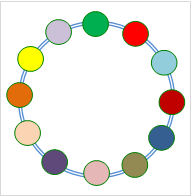
\includegraphics[scale=.6, keepaspectratio]{content/math/Burnside-Necklace.png}
    \end{center}
	$$\frac{1}{n} \sum_{i=1}^n k^{\gcd(i, n)}$$

	\textbf{Example2:} Count the number of different n $\times$ n grids whose each square is black or white.

	Two grids are considered to be different if it is not possible to rotate one of them so that they look the same.
	
	\begin{center}
	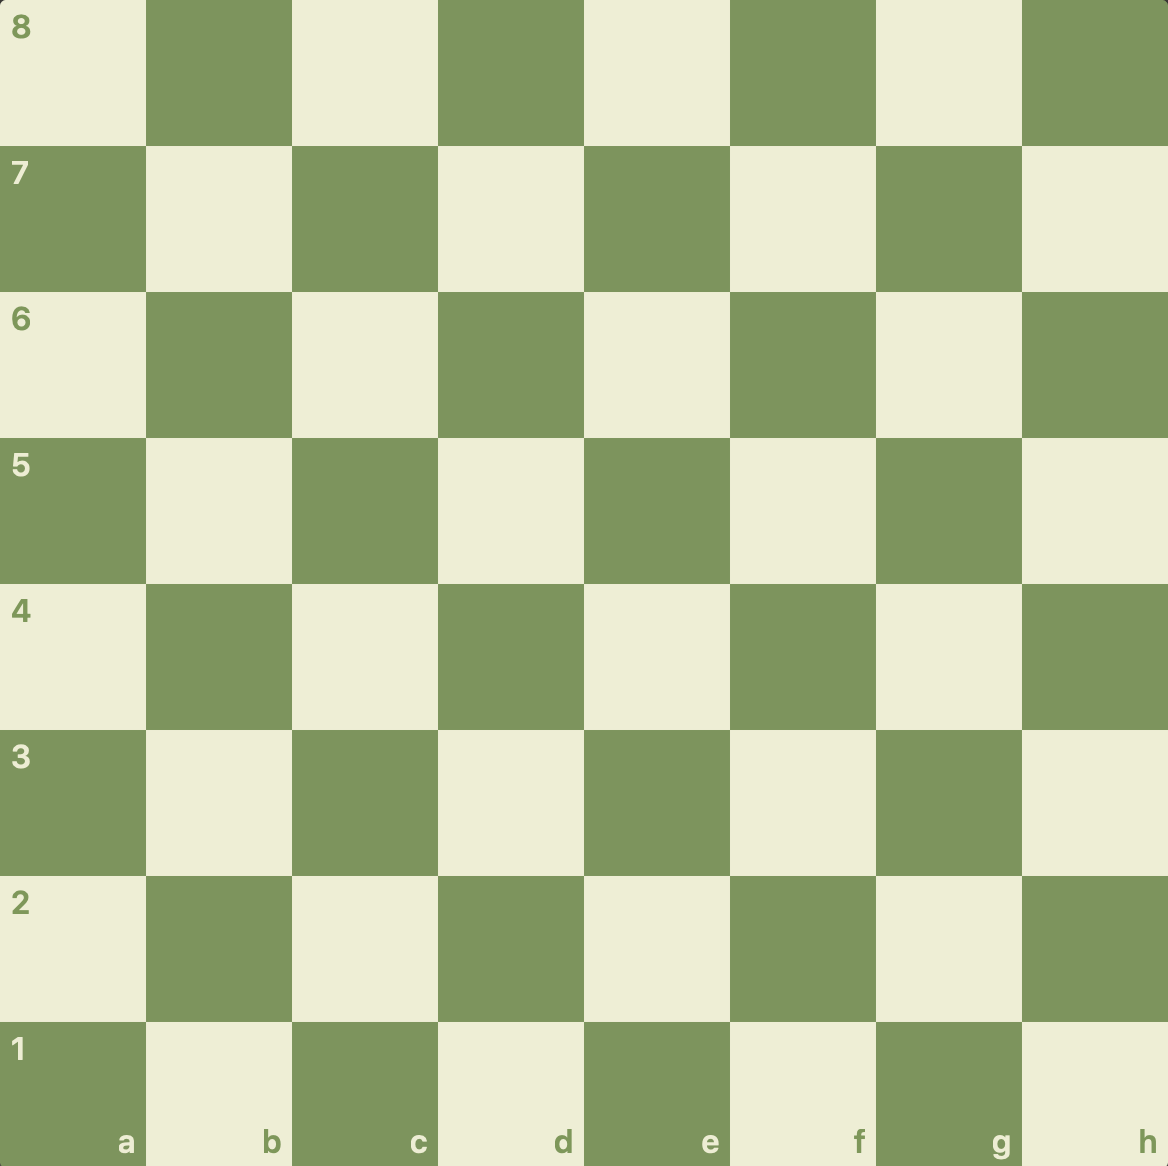
\includegraphics[scale=.1, keepaspectratio]{content/math/Burnside-Grid.png}
	\end{center}

	$$ G (Rotations) = 0^{\circ}, 90^{\circ}, 180^{\circ}, 270^{\circ} $$

	\begin{centering}
	\begin{align*}
	f(rotation) = & \\
	0^{\circ}: 				& 2^{(n^2)}  \\
	90^{\circ}/270^{\circ}:	& 2^{ \frac{n^2}{4} }, & n_{even} \\
							& 2^{ \frac{n^2-1}{4} } \cdot 2 , & n_{odd} \\
	180^{\circ}:			& 2^{ \frac{n^2}{2} }, & n_{even} \\
							& 2^{ \frac{n^2-1}{2} } \cdot 2 , & n_{odd}
	\end{align*}
	\end{centering}

	
	$$ans = \frac{1}{4} (f(0^{\circ}) + f(90^{\circ}) + f(180^{\circ}) + f(270^{\circ})) $$

	\subsection{Interesting Recursion}

	$$ f(a, b) = f(a-1, b) + f(a, b-1) $$

	$$ \implies f(a, b) = \frac{(a+b)!}{a! b!} = \binom{a+b}{a} $$

	\textit{Proof:}
	
	\begin{align*}
	&f(a, b) = \frac{(a+b)!}{a! b!}  \\ 
	\implies &f(a-1, b) = \frac{(a-1+b)!}{(a-1)! b!}, f(a, b-1) = \frac{(a+b-1)!}{a! (b-1)!}  \\
	\implies &f(a-1, b) + f(a, b-1) = \frac{(a-1+b)!}{(a-1)! b!} + \frac{(a+b-1)!}{a! (b-1)!}  \\
	\implies &f(a, b) = (a+b-1)! \cdot ( \frac{1}{(a-1)!(b)!} + \frac{1}{(a)!(b-1)!} )  \\
	\implies &f(a, b) = (a+b-1)! \cdot ( \frac{a+b}{a! b!} ) \\
	\implies &f(a, b) = \frac{(a+b)!}{a! b!} = \binom{a+b}{a} 
	\end{align*}

\section{FFT}

	FFT can be used to turn a polynomial multiplication complexity to $O(N \log{N})$.

	A \textbf{convulution} is easily computed by inverting the second vector and doing the polynomial multiplication normally.

	\kactlimport{fft-simple.cpp}

\section{Matrix}

For faster linear recurrence computation with matrix exponentiation. 

$$ Base * Operator^{k} = Result $$

\kactlimport{matrix.cpp}